\documentclass[12pt]{article}
\usepackage[all, stdclass]{lix}
\usepackage{graphicx}
\usepackage{svg}
\svgsetup{
  inkscapepath=assets/,  % Path to the directory containing your SVG files
  svgpath=assets/        % Path to the directory containing your SVG files
}
\usepackage{float}
\usepackage{hyperref}
\usepackage{times}
\usepackage{amsmath}

% /main/2023-08-23-18-08-17.png - Carrier Profile
% /main/2023-08-23-18-26-49.png - Modulation
% /main/2023-08-23-18-27-00.png - Demodulation1
% /main/2023-08-23-18-27-58.png - Both Modulation and Demodulation1
% /main/2023-08-23-18-30-59.png - System

%----------EDIT COVER INFO HERE -----------------%

\def \LOGOPATH {assets/birzeit-logo.png}
\def \DEPARTEMENT {Department of Electrical \& Computer Engineering}
\def \COURSENUM {ENEE4113}
\def \COURSENAME {Communications Laboratory}
\def \REPORTTITLE {Frequency Shift Keying (FSK) and Phase Shift Keying (PSK)}
\def \STUDENTNAME {Mohammad Abu-Shelbaia}
\def \STUDENTID {1200198}
\def \INSTRUCTOR {Dr. Ibrahim Nemer}
\def \ASSISTANT {Eng. Mohammad Al-Battat}
\def \REPORTNUM {11}

\begin{document}
\pagenumbering{Roman}

\begin{titlepage}
    \vfill
    \begin{center}
        \includegraphics[width=0.7\textwidth]{\LOGOPATH} \\
        \hfill \\
        \Large{\DEPARTEMENT} \\
        \Large{\COURSENUM\;-\;\COURSENAME} \\
        \vfill
        \textbf{\LARGE{Experiment \#\REPORTNUM}} \\
        \textbf{\LARGE{\REPORTTITLE}}
    \end{center}
    \vfill
    \begin{flushleft}
        \Large{\textbf{Prepared by:}\\ \STUDENTNAME\quad\STUDENTID} \\

        \Large{\textbf{Instructor:} \INSTRUCTOR} \\
        \Large{\textbf{Assistant:} \ASSISTANT} \\
        \Large{\textbf{Section:} 4}\\
        \LARGE{\textbf{ }}\\
        \LARGE{\textbf{ }}\\
        \LARGE{\textbf{ }}\\
        \Large{\textbf{Date:} \today}\\
    \end{flushleft}
    \vfill
\end{titlepage}


%--------------- TABLES --------------------------------%
\tableofcontents
\clearpage
\setlength{\parskip}{\baselineskip}%
\listoffigures
\clearpage
% \listoftables
% \clearpage
\pagenumbering{arabic}
%-------------- CONTENT ---------------------%
\h{Simulation and Data Analysis}
\hh{Frequency Shift Keying (FSK)}
\begin{figure}[H]
    \centering
    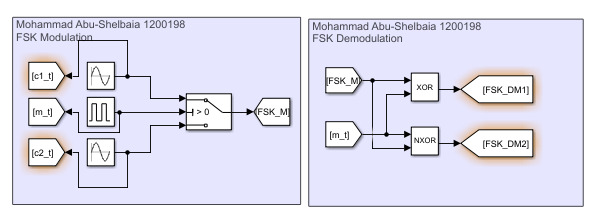
\includegraphics[width=1\textwidth]{assets/main/2023-08-27-14-39-32.png}
    \caption{Modulation/Demodulation Simulink Block Diagram}
\end{figure}
The above system is simulated using MATLAB Simulink for different messages modulated over two carrier signal:
\begin{equation}
    c(t) = \cos(2\pi(15k)t)
\end{equation}
\begin{equation}
    c(t) = \cos(2\pi(25k)t)
\end{equation}
\hhh{Input Signals}

\begin{figure}[H]
    \centering
    \resizebox{0.49\textwidth}{0.23\textwidth}{
        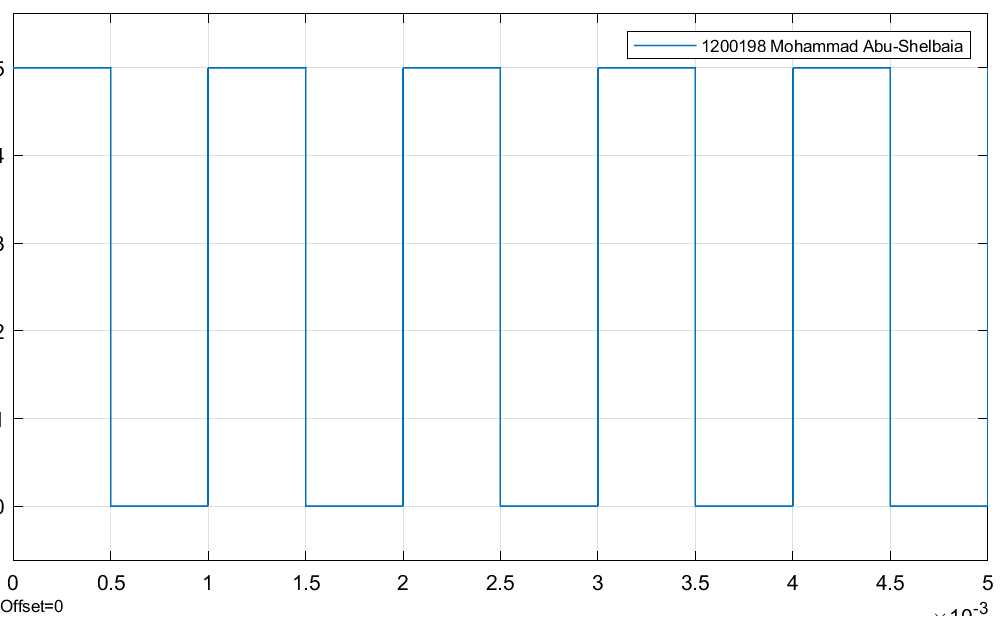
\includegraphics[width=\textwidth]{assets/main/2023-08-23-18-56-06.png}
    }
    \resizebox{0.49\textwidth}{0.23\textwidth}{
        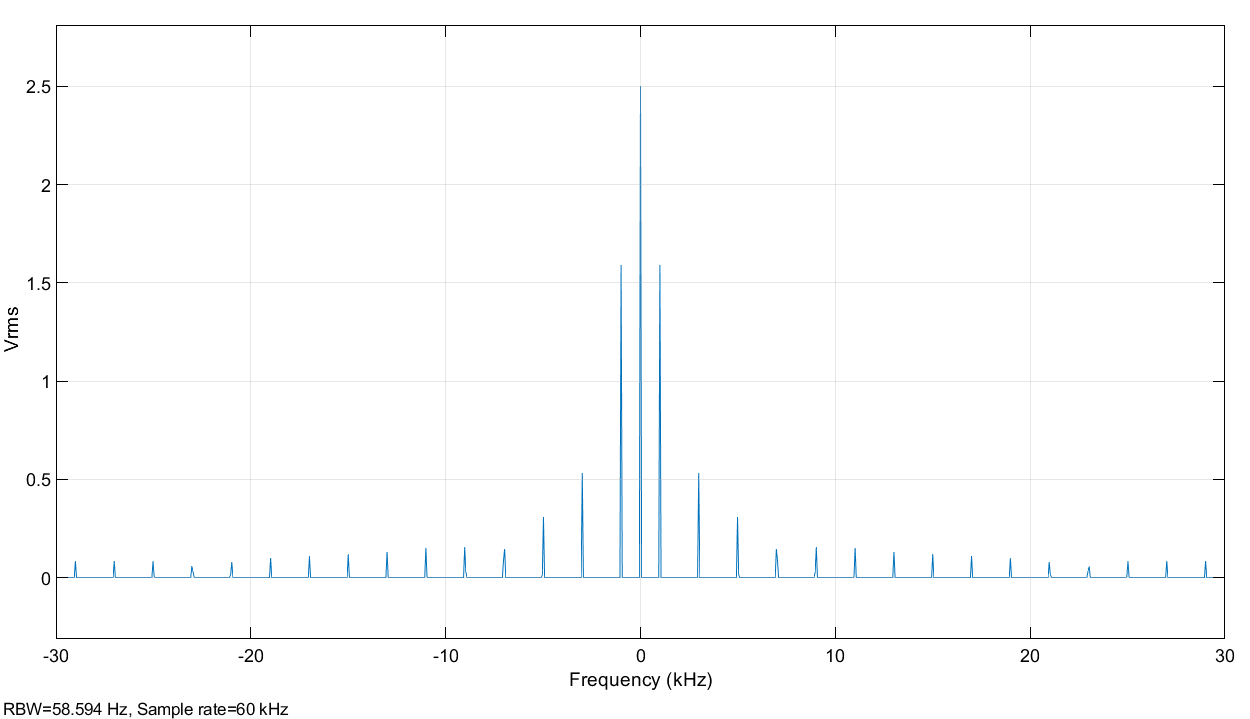
\includegraphics[width=\textwidth]{assets/main/2023-08-23-19-13-47.png}
    }
    \caption{Message Signal}
\end{figure}
\begin{figure}[H]
    \centering
    \resizebox{0.49\textwidth}{0.23\textwidth}{
        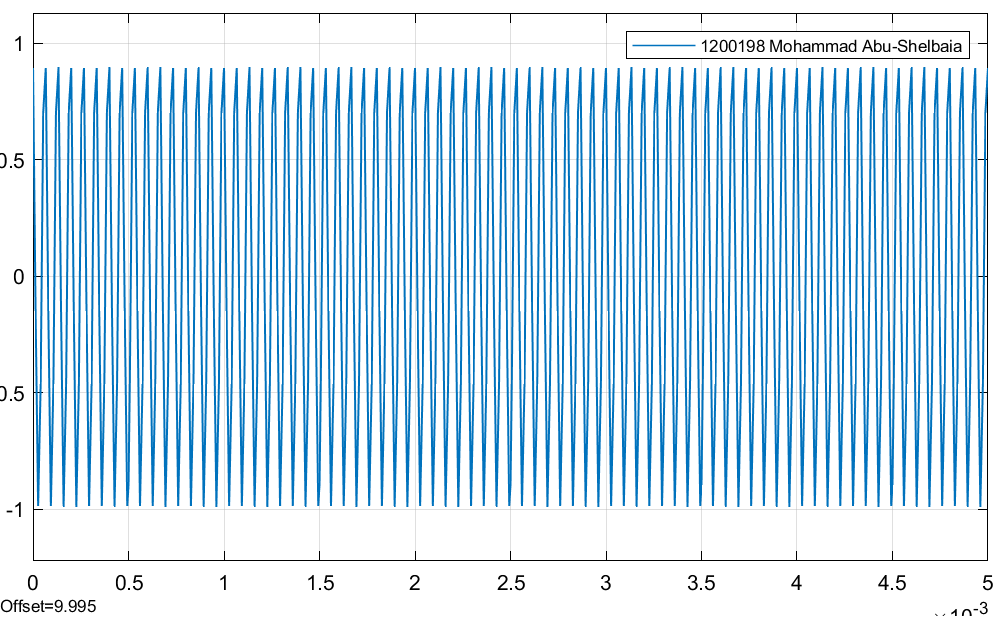
\includegraphics[width=\textwidth]{assets//main/2023-08-27-14-45-47.png}
    }
    \resizebox{0.49\textwidth}{0.23\textwidth}{
        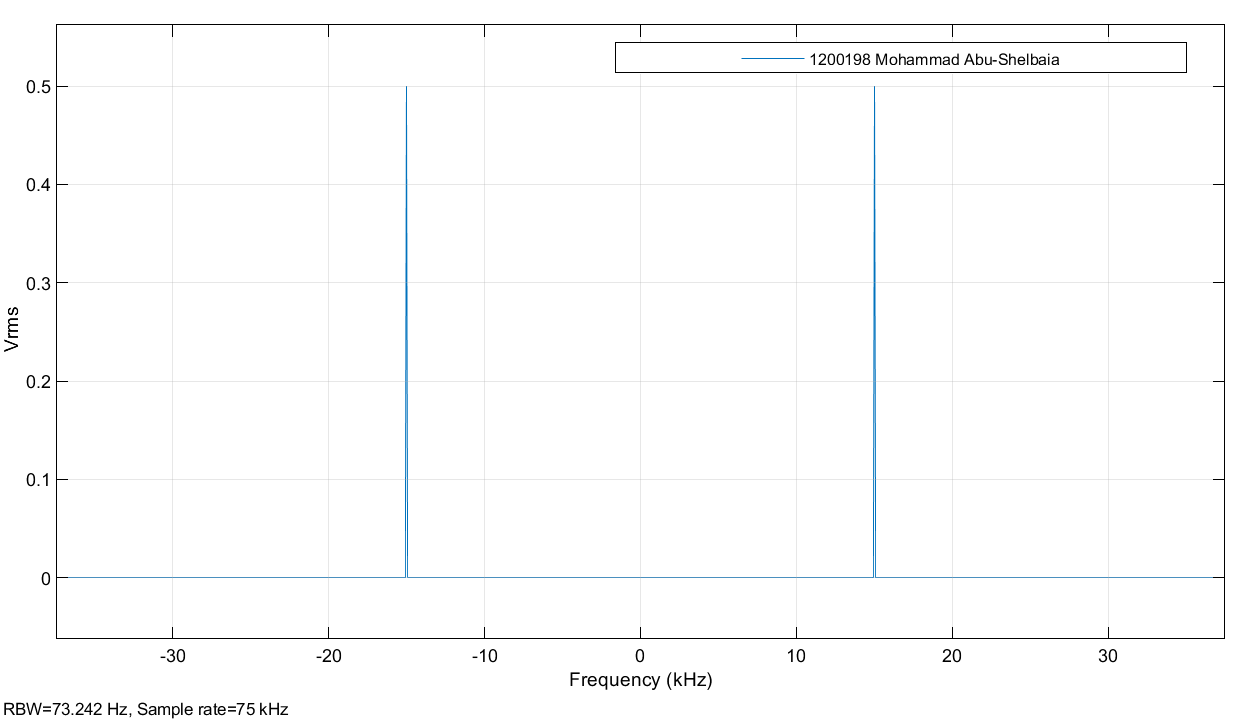
\includegraphics[width=\textwidth]{assets//main/2023-08-27-14-46-27.png}
    }
    \caption{Carrier1 Signal}
\end{figure}
\begin{figure}[H]
    \centering
    \resizebox{0.49\textwidth}{0.23\textwidth}{
        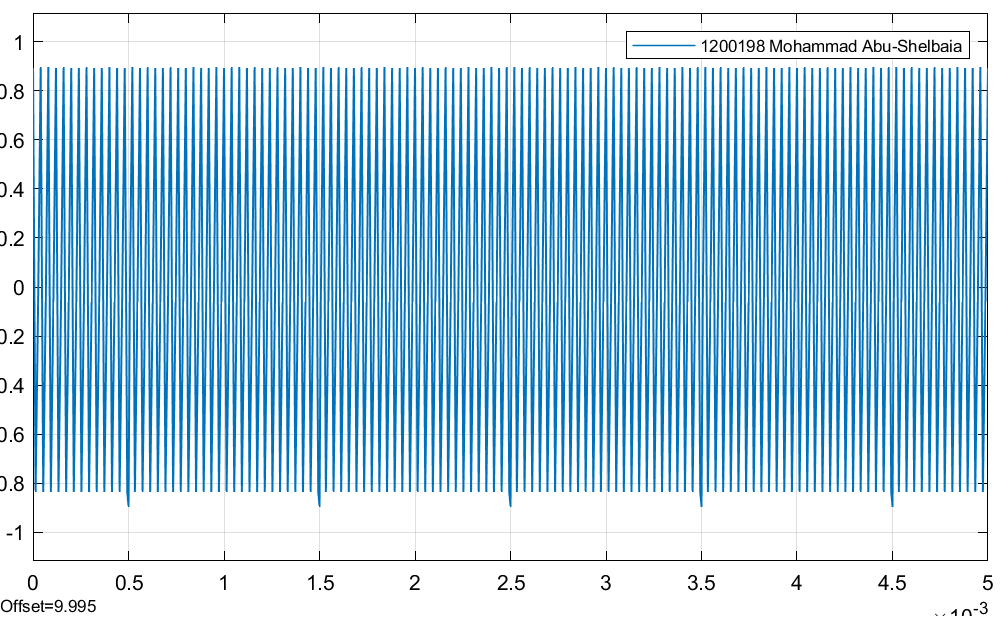
\includegraphics[width=\textwidth]{assets//main/2023-08-27-14-46-15.png}
    }
    \resizebox{0.49\textwidth}{0.23\textwidth}{
        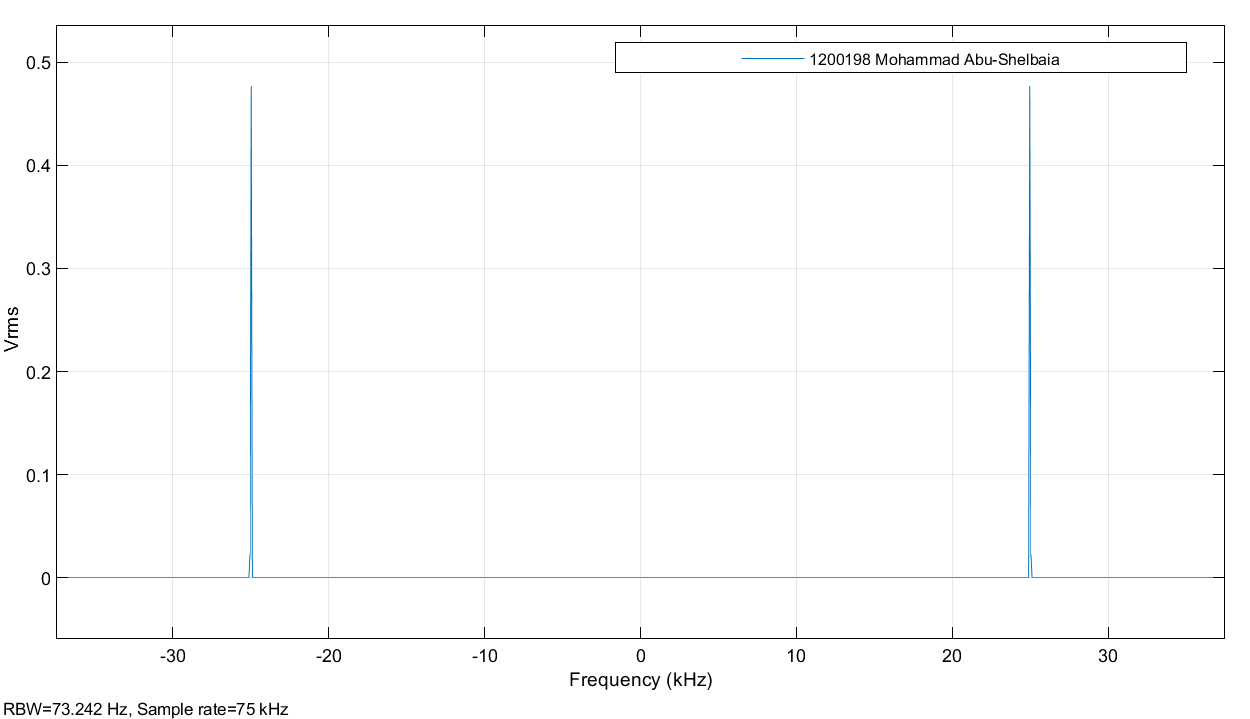
\includegraphics[width=\textwidth]{assets//main/2023-08-27-14-46-46.png}
    }
    \caption{Carrier2 Signal}
\end{figure}
\hhh{Modulation and Demodulation}
\textbf{Refrence Modulating Signal}
This is our refrence modulating signal, which is a pulse-train with a frequency of 1KHz, duty cycle of 50\%, and an amplitude of 5V.
\begin{figure}[H]
    \centering
    \resizebox{0.49\textwidth}{0.25\textwidth}{
        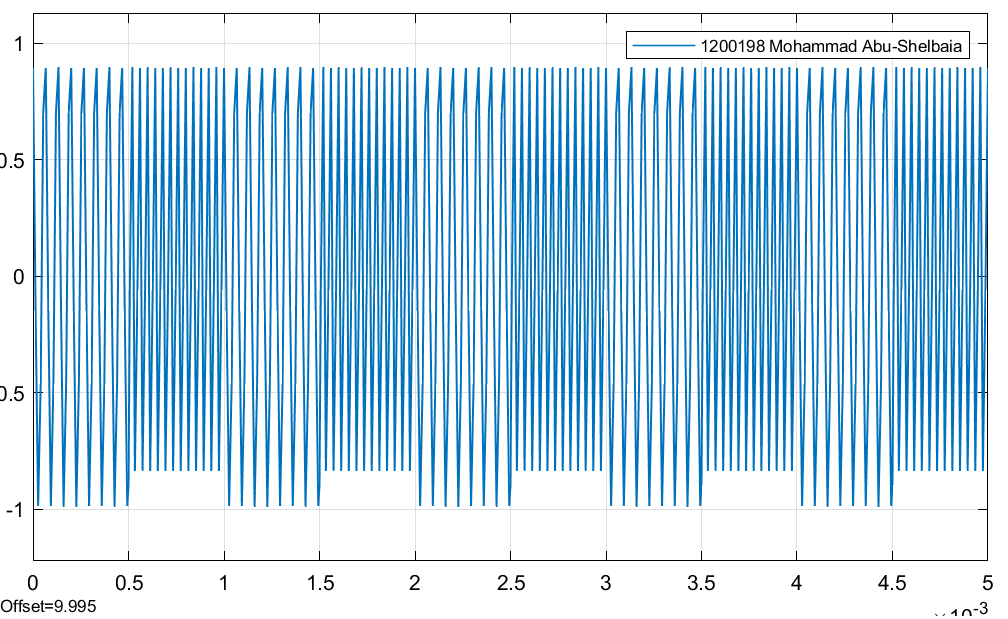
\includegraphics[width=\textwidth]{assets//main/2023-08-27-14-51-24.png}
    }
    \resizebox{0.49\textwidth}{0.25\textwidth}{
        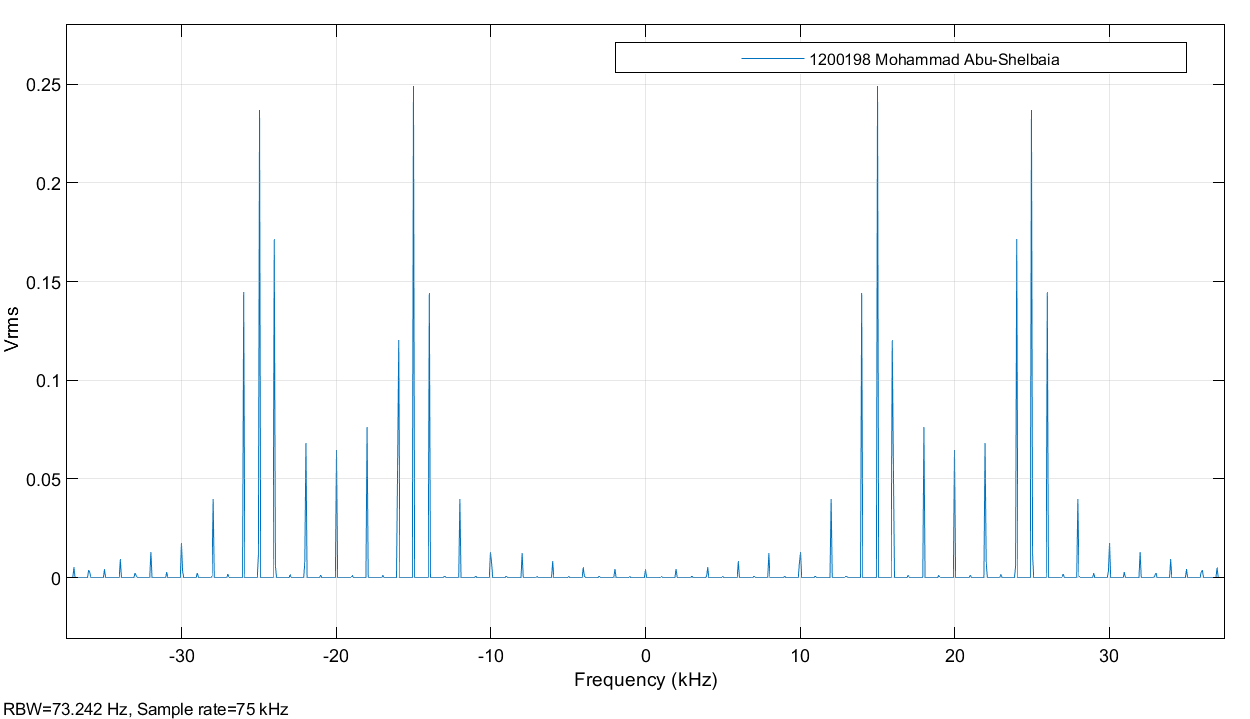
\includegraphics[width=\textwidth]{assets//main/2023-08-27-14-51-47.png}
    }
    \caption{Modulated Singal}
\end{figure}
We can see that the modulated signal is a cosine wave with two different frequencies, 15KHz and 25KHz, each frequency is used to represent a bit, 0 or 1, the high frequency is used to represent 0, and the low frequency is used to represent 1.
\begin{figure}[H]
    \centering
    \resizebox{0.49\textwidth}{0.25\textwidth}{
        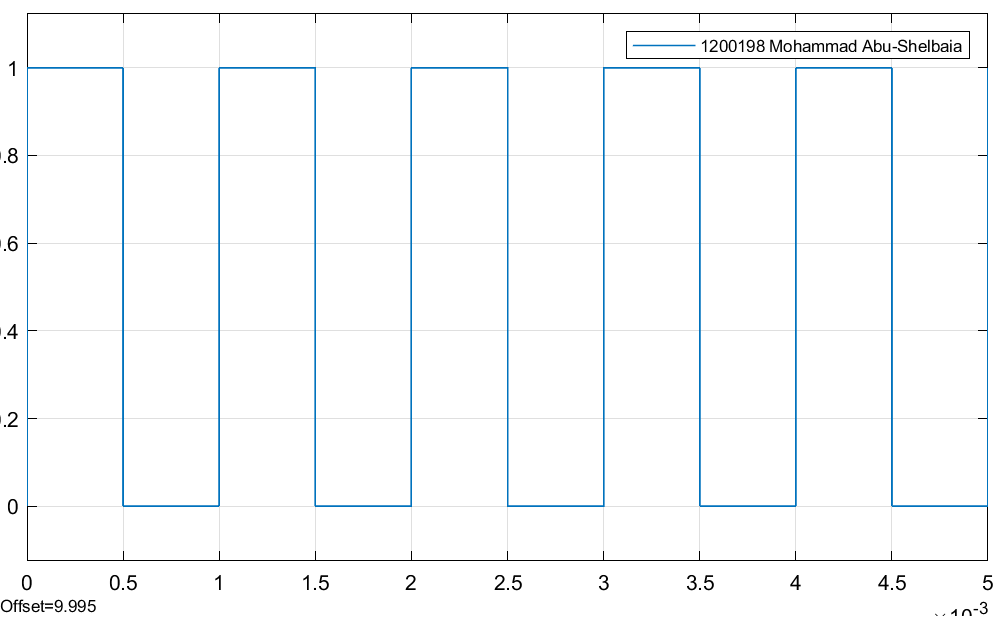
\includegraphics[width=\textwidth]{assets/main/2023-08-27-14-55-35.png}
    }
    \resizebox{0.49\textwidth}{0.25\textwidth}{
        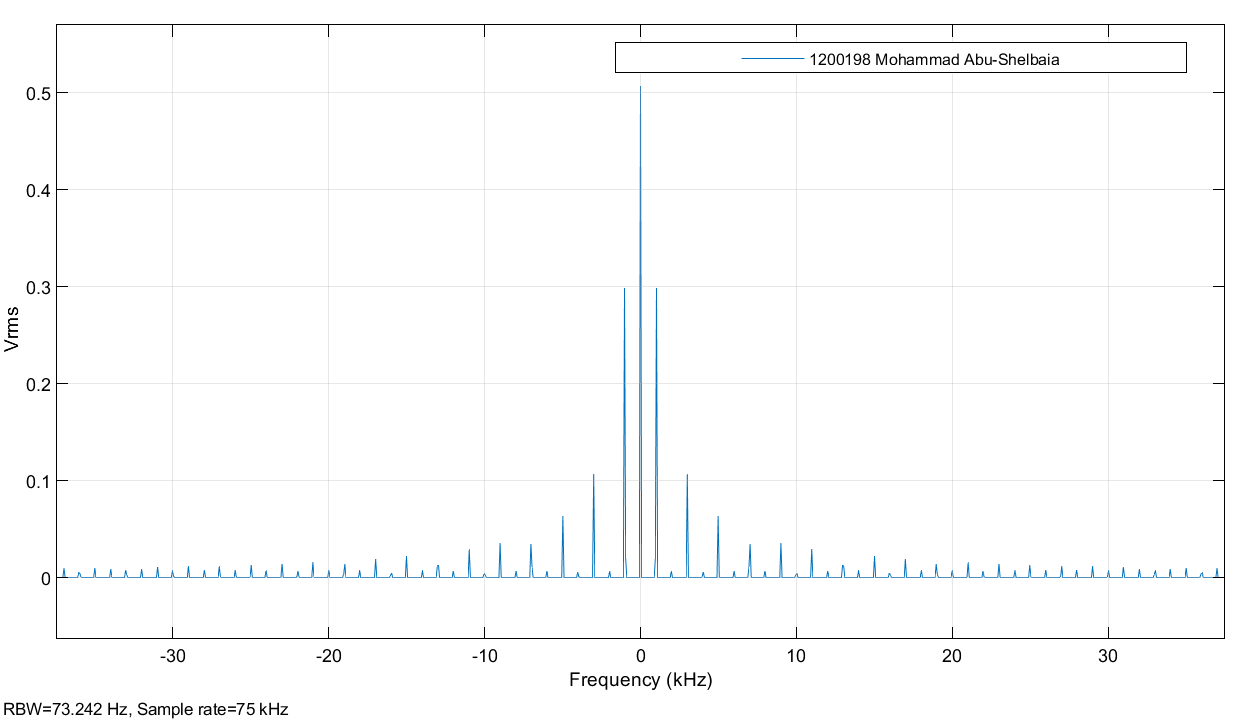
\includegraphics[width=\textwidth]{assets/main/2023-08-27-14-56-11.png}
    }
    \caption{Demodulaed Singal}
\end{figure}
We can see that we have successfully demodulated the signal using both methods, the high portion of the message singal is recoverd as 1, and the low portion is recovered as 0.
\textbf{2V Modulating Signal}
\begin{figure}[H]
    \centering
    \resizebox{0.49\textwidth}{0.25\textwidth}{
        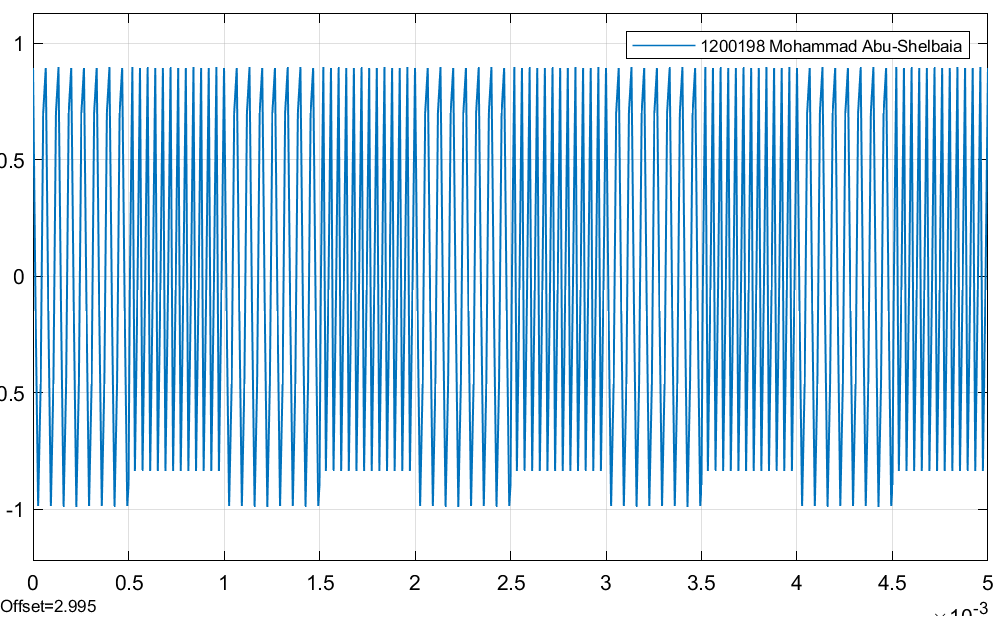
\includegraphics[width=\textwidth]{assets//main/2023-08-27-14-58-51.png}
    }
    \resizebox{0.49\textwidth}{0.25\textwidth}{
        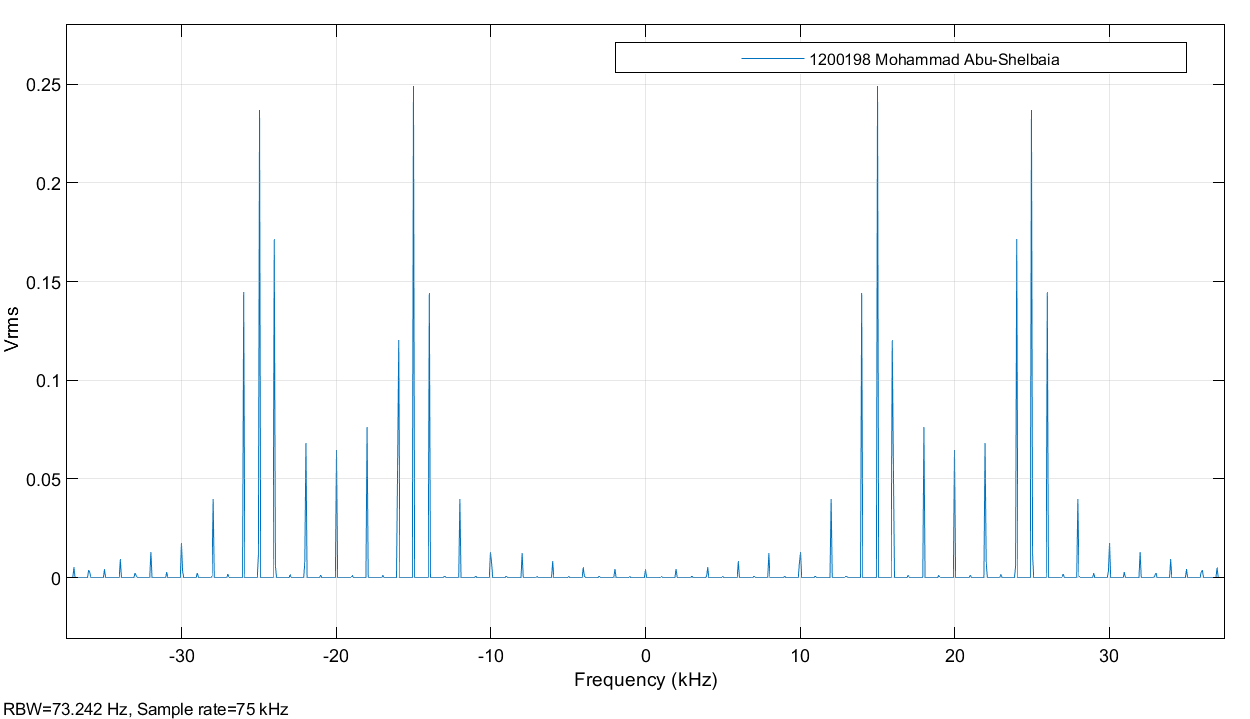
\includegraphics[width=\textwidth]{assets//main/2023-08-27-14-59-12.png}
    }
    \caption{Modulated Singal (2V)}
\end{figure}
We can see that the amplitude of the modulating signal does not affect the modulated signal.
\begin{figure}[H]
    \centering
    \resizebox{0.49\textwidth}{0.25\textwidth}{
        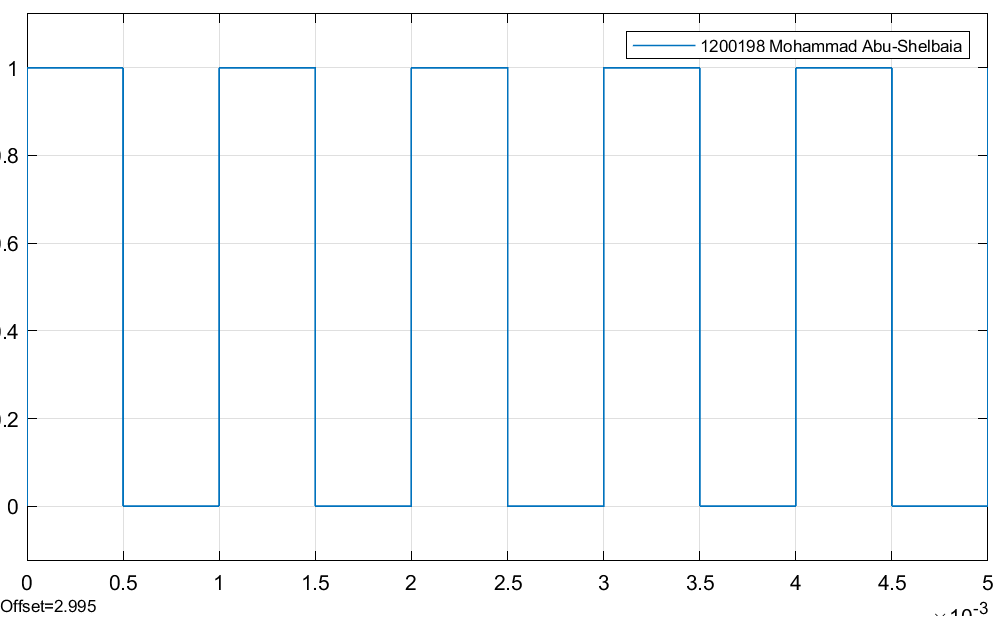
\includegraphics[width=\textwidth]{assets//main/2023-08-27-14-59-43.png}
    }
    \resizebox{0.49\textwidth}{0.25\textwidth}{
        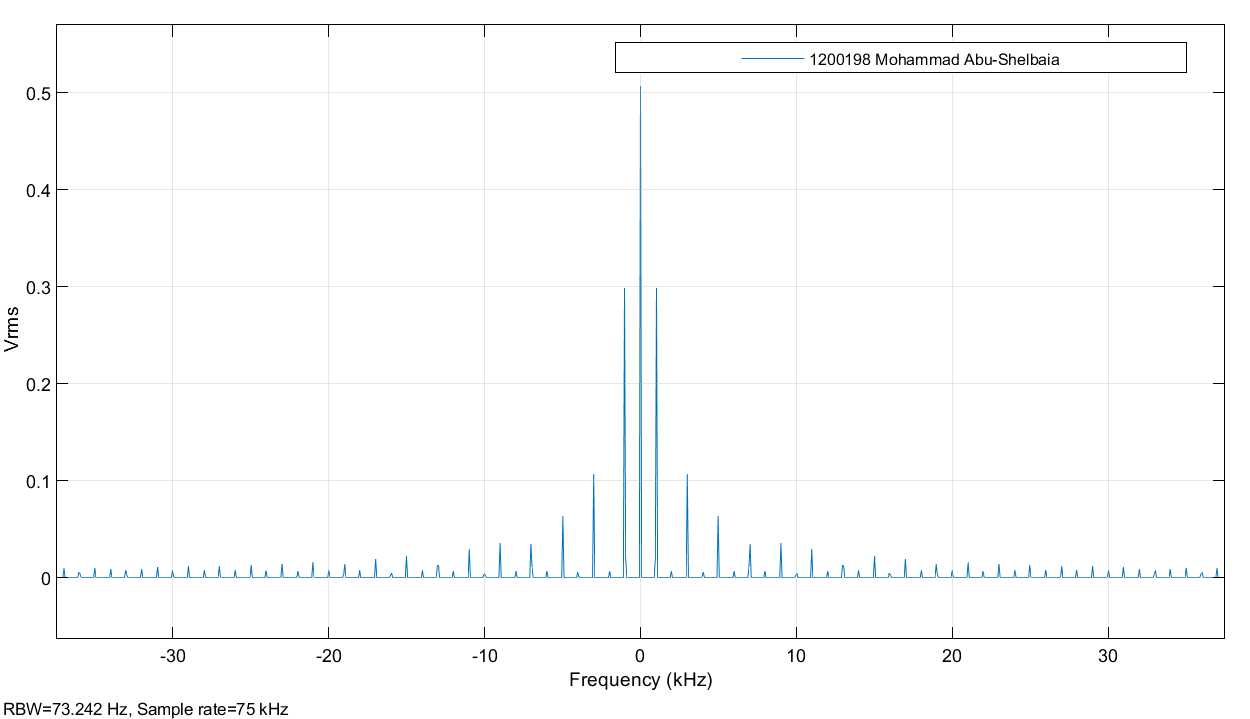
\includegraphics[width=\textwidth]{assets//main/2023-08-27-14-59-36.png}
    }
    \caption{Demodulated Singal (2V)}
\end{figure}

We can see the same results as before, and we conclude that the amplitude of the modulating signal does not affect the demodulation process. \\
\textbf{500Hz Modulating Signal}
\begin{figure}[H]
    \centering
    \resizebox{0.49\textwidth}{0.25\textwidth}{
        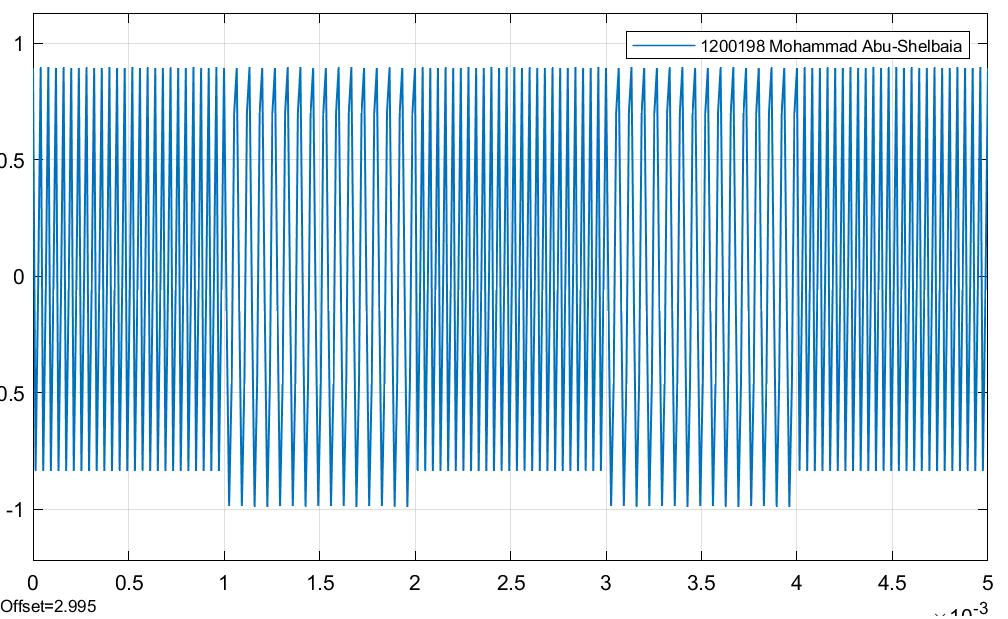
\includegraphics[width=\textwidth]{assets/main/2023-08-27-15-07-58.png}
    }
    \resizebox{0.49\textwidth}{0.25\textwidth}{
        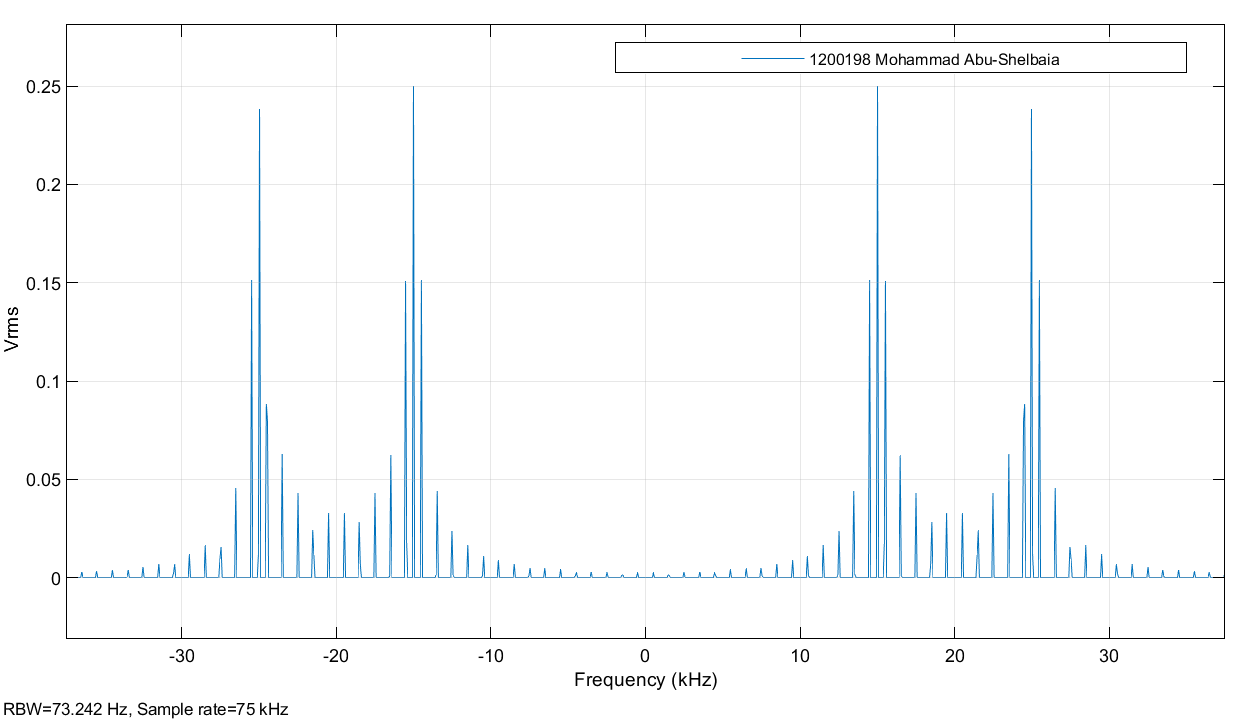
\includegraphics[width=\textwidth]{assets/main/2023-08-27-15-08-09.png}
    }
    \caption{Modulated Singal (500Hz)}
\end{figure}
\begin{figure}[H]
    \centering
    \resizebox{0.49\textwidth}{0.25\textwidth}{
        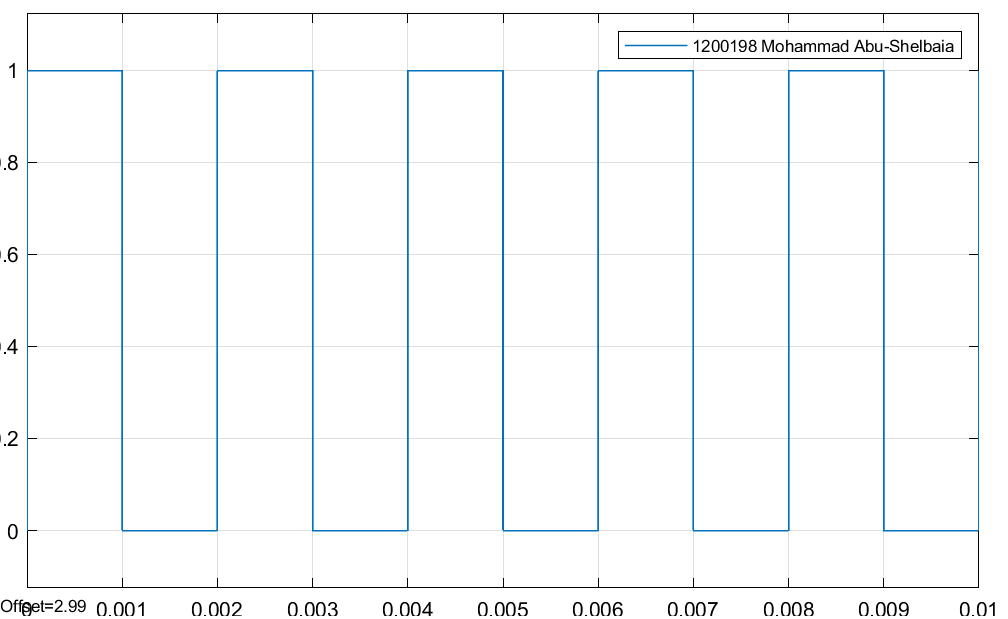
\includegraphics[width=\textwidth]{assets//main/2023-08-27-15-16-04.png}
    }
    \resizebox{0.49\textwidth}{0.25\textwidth}{
        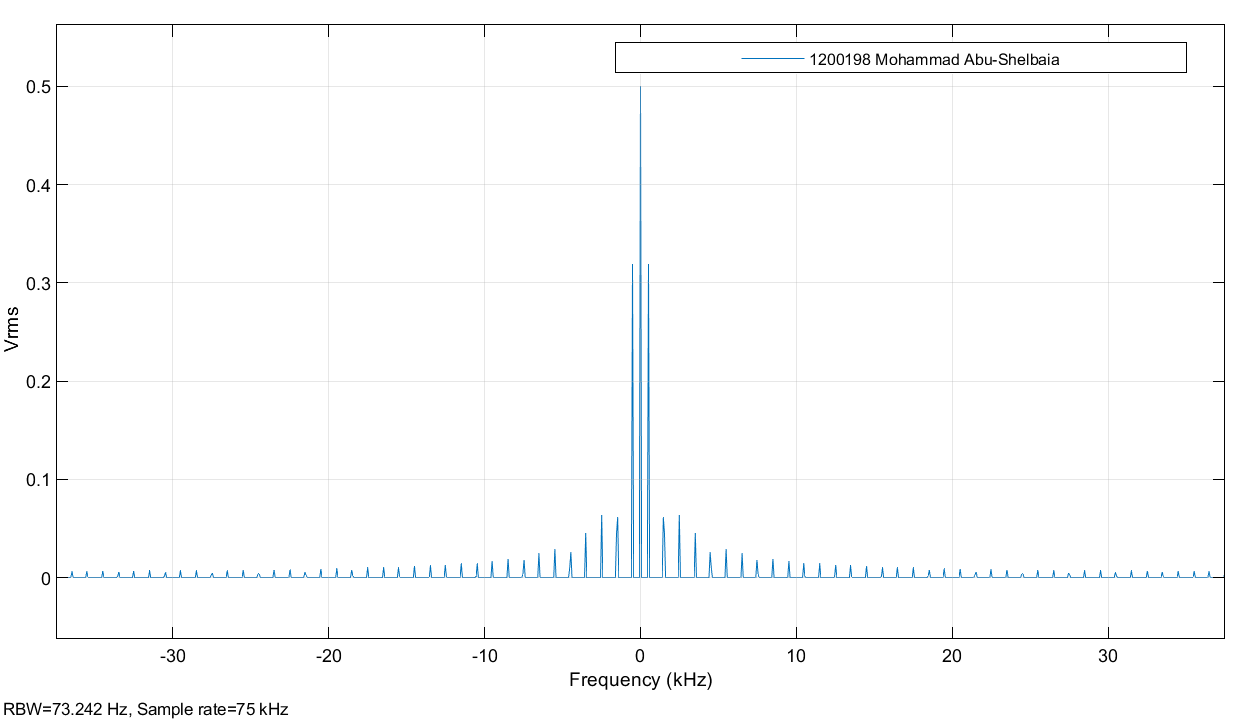
\includegraphics[width=\textwidth]{assets//main/2023-08-27-15-08-24.png}
    }
    \caption{Demodulated Singal (500Hz)}
\end{figure}
Here the freqeuncy deviation (The space between pulses) is lower which saves bandwidth. \clearpage
\textbf{0.10 Duty-Cycle Modulating Signal}
\begin{figure}[H]
    \centering
    \resizebox{0.49\textwidth}{0.25\textwidth}{
        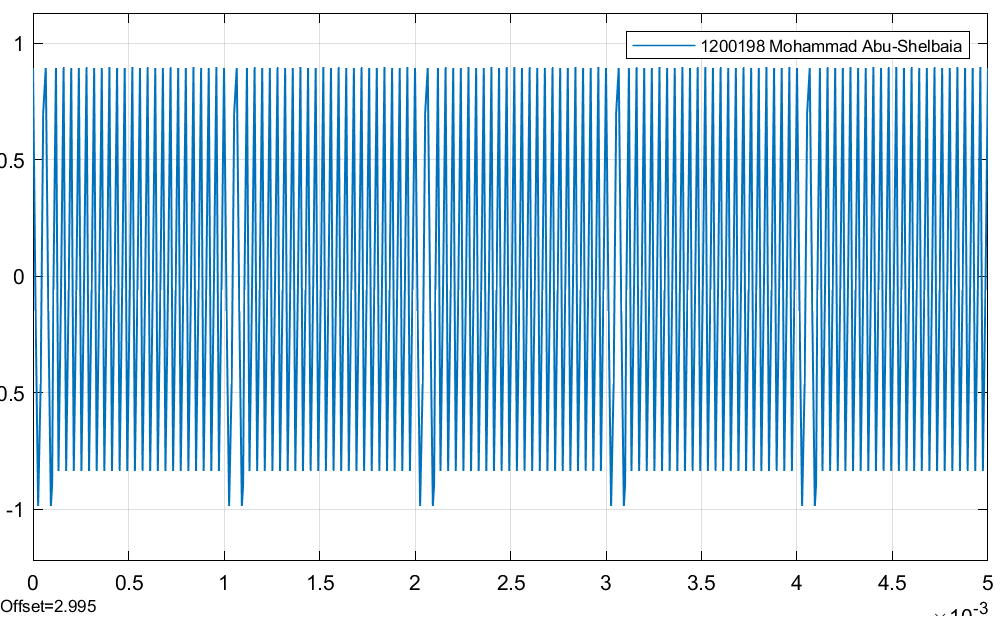
\includegraphics[width=\textwidth]{assets//main/2023-08-27-15-19-38.png}

    }
    \resizebox{0.49\textwidth}{0.25\textwidth}{
        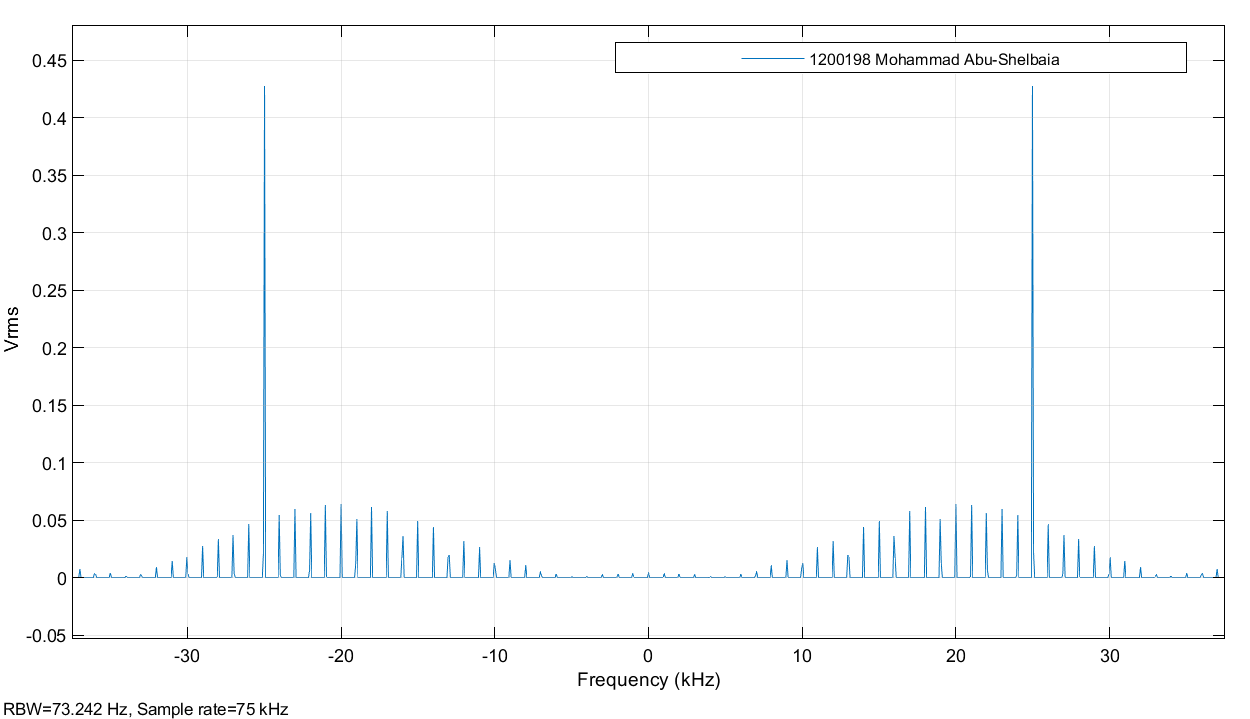
\includegraphics[width=\textwidth]{assets//main/2023-08-27-15-19-59.png}

    }
    \caption{Modulated Singal (10\% Duty Cycle)}
\end{figure}
We notice that the duty cycle of the modulating signal does not affect the modulated signal in simulation but it might affect it in real life since it looks like a noise to the modulated signal.
\begin{figure}[H]
    \centering
    \resizebox{0.49\textwidth}{0.25\textwidth}{
        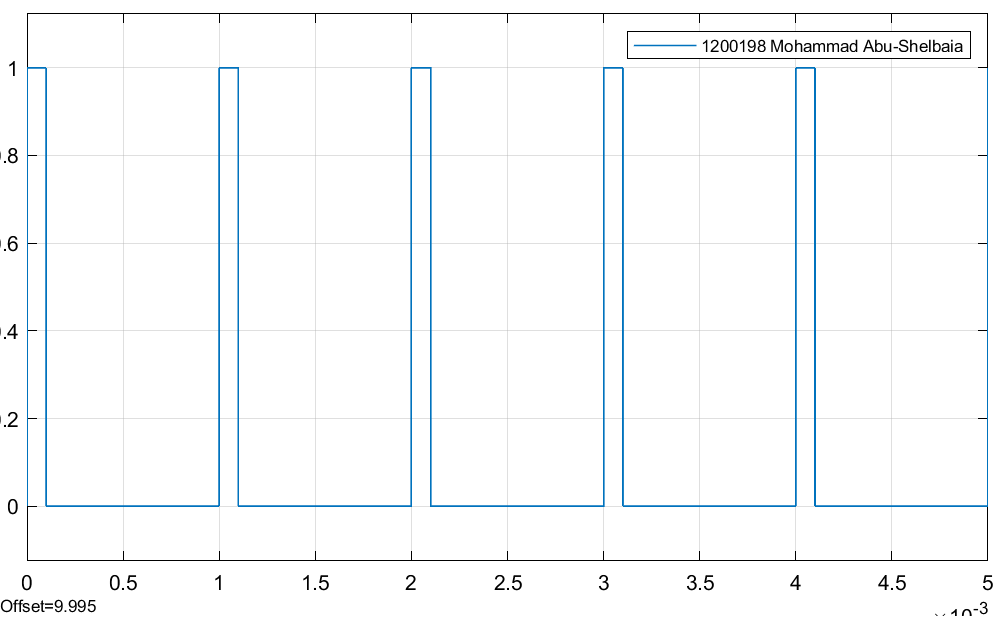
\includegraphics[width=\textwidth]{assets/main/2023-08-23-20-16-16.png}
    }
    \resizebox{0.49\textwidth}{0.25\textwidth}{
        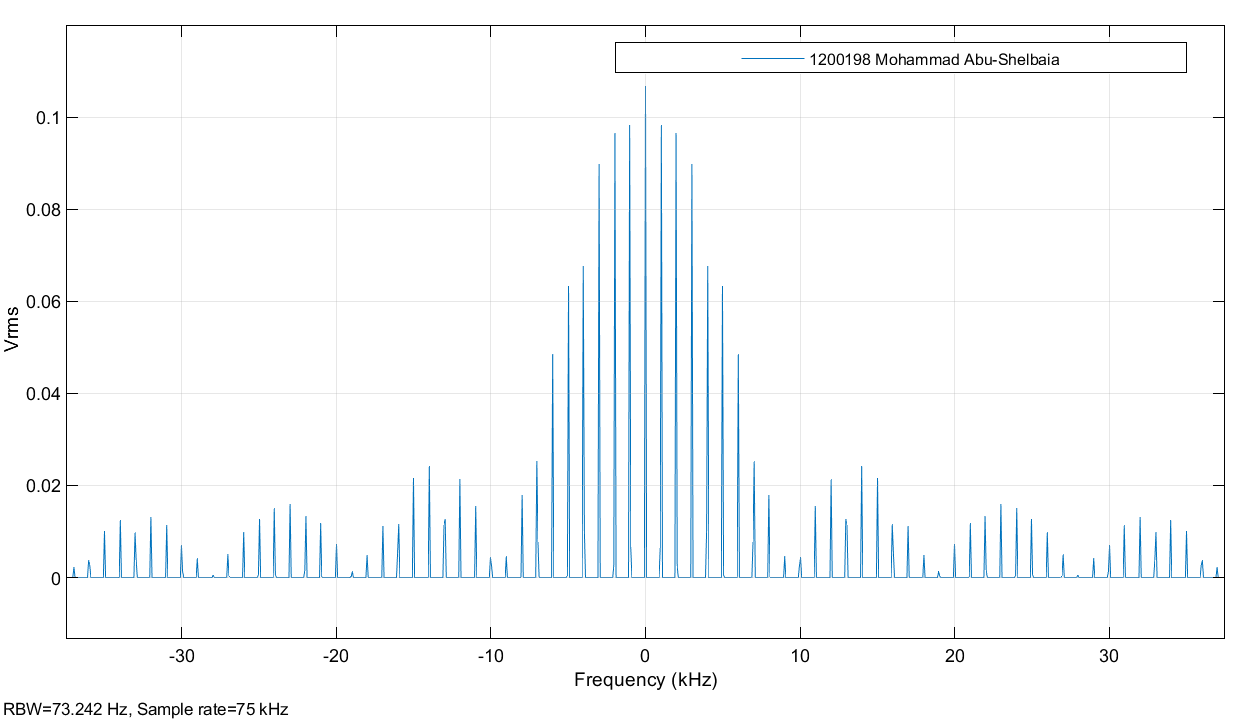
\includegraphics[width=\textwidth]{assets//main/2023-08-27-15-20-24.png}
    }
    \caption{Demodulated Singal (10\% Duty Cycle)}
\end{figure}
We can see as all the previous parts we were able to recover the message correctly, the high portion of the message singal is recoverd as one, and the low portion is recovered as zero.
\hh{Phase Shift Keying (PSK)}
\begin{figure}[H]
    \centering
    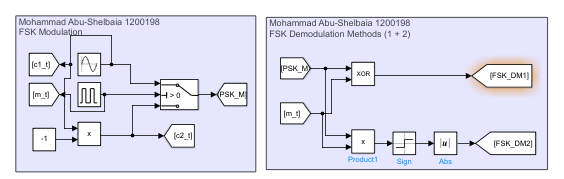
\includegraphics[width=1\textwidth]{assets//main/2023-08-27-16-46-40.png}
    \caption{Modulation/Demodulation Simulink Block Diagram}
\end{figure}
The above system is simulated using MATLAB Simulink for different messages modulated over one carrier signal with a phase shift of 180 degrees:
\begin{equation}
    c(t) = \cos(2\pi(20k)t)
\hhh{Input Signals}

\end{equation}
\end{document}





